\documentclass[aps,prb,twocolumn,letterpaper,twoside,nobalancelastpage,groupedaddress,amsmath,amssymb,floatfix,citeautoscript]{revtex4-1}
%\usepackage{geometry}       
%\geometry{letterpaper}     
%\usepackage[parfill]{parskip}    % Activate to begin paragraphs with an empty line rather than an indent
\usepackage{graphicx}
\usepackage{bm} %bold math symbols
\usepackage{times}
\usepackage{graphicx}
\usepackage{physics}
\usepackage{outlines}             
\usepackage{amssymb}
\usepackage[caption=false]{subfig}
\usepackage{mathtools}
\usepackage{color}
\definecolor{darkred}{rgb}{0.6,0.,0.}
\definecolor{darkgreen}{rgb}{0.,0.5,0.}
\definecolor{darkblue}{rgb}{0.,0.,0.6}

\usepackage{framed}

%\usepackage[square,numbers,sort,merge]{natbib}
\usepackage[
breaklinks,
colorlinks=true,
linkcolor=darkred,
citecolor=darkgreen,
urlcolor=darkblue]{hyperref}
%\usepackage{doi}

% \DeclareMathOperator{\tr}{tr}
% \DeclareMathOperator{\erf}{Erf}

\DeclareGraphicsRule{.tif}{png}{.png}{`convert #1 `dirname #1`/`basename #1 .tif`.png}

\begin{document}


\def \Ns {\mathbb{N}}
\def \Rs {\mathbb{R}}
\def \Zs {\mathbb{Z}}
\def \Qs {\mathbb{Q}}
\def \Cs {\mathbb{C}}
\def \id {\mathbb{I}}

\def \bfq {{\bf q}}
\def \bfp {{\bf p}}
\def \bfx {{\bf x}}
\def \bfy {{\bf y}}
\def \bfz {{\bf z}}
\def \bfr {{\bf r}}
\def \bfk {{\bf k}}
\def \bfn {{\bf n}}
\def \bfb {{\bf b}}
\def \bfm {\mathbf{m}}
\def \bfn {\mathbf{n}}

%\def \hata {{a}}
%\def \hatadag {{a}^{\dagger}}

\def \hatq {\widehat{q}}
\def \hatp {\widehat{p}}
\def \hata {\widehat{a}}
\def \hatadag {\widehat{a}^{\dagger}}
%\def \hatb {\widehat{b}^\phantom{\dagger}}
%\def \hatbdag {\widehat{b}^{\dagger}}
\def \wtN {\widetilde{N}}

\def \ve {\varepsilon}
\def \vth {\vartheta}



\title{Lattice models for generic Landau orbits}
\author{David Bauer}
\email{dbauer@physics.ucla.edu}
\affiliation{Department of Physics and Astronomy, University of California at Los Angeles, 475 Portola Plaza, Los Angeles, California 90095, USA}

\author{Fenner Harper}
\affiliation{Department of Physics and Astronomy, University of California at Los Angeles, 475 Portola Plaza, Los Angeles, California 90095, USA}

\author{Rahul Roy}
\affiliation{Department of Physics and Astronomy, University of California at Los Angeles, 475 Portola Plaza, Los Angeles, California 90095, USA}

\date{\today}
\begin{abstract}
Abstract goes here.
 
\end{abstract}

% \pacs{0}

\maketitle

\section{Introduction}
[In progress...]


\section{Review}
\subsection{Background and motivation}
The incompressible liquid phases of the fractional quantum Hall (FQH) effect serve as prototypical examples of topologically ordered or gapped quantum liquid phases\cite{YoshiokaBook,FradkinBook}. Two recent developments in FQH physics have each inspired a large body of literature. The first is the discovery of fractional Chern insulators (FCI), which are fractionalized phases of interacting particles in the presence of a strong lattice potential\cite{Bergholtz:2013ue,Parameswaran2013}. This is in contrast to the traditional picture of the quantum Hall effect, which is formulated in the continuum. Research on the FQHE in the presence of a lattice potential has a long history \cite{Kol:1993hs,Sorensen:2005bt,Palmer2006}. However, FCIs redoubled interest in this field with the potential for realizing FQH phases in novel experimental settings. The distinction between FCI models and the more traditional Harper-Hofstadter \cite{Harper:1955ft,Azbel:1964tk,Hofstadter:1976js} models for lattice electron gasses is nominally that the former have no \textit{net} magnetic field per unit cell. However this distinction is unecessary from a theoretical point of view\cite{McGreevy2012}, and we view FCIs simply as the limit of Harper-Hofstadter models when lattice effects are strong.

A second development in the FQH literature is based on observations that, in spite of their topological nature, FQH liquids are also characterized by non-trivial geometrical properties, including the Hall viscosity\cite{Avron:1985fo,Read2009} and thermal Hall conductivity or gravitational anomaly\cite{Luttinger1964,Kane1997,CAPPELLI2002568,Stone2012}. These two lines of inquiry are related in that the addition of a non-negligible lattice potential introduces additional geometric data that may break some non-generic symmetries. For example, in the case of a square lattice, $SO(2)$ rotational invariance in the coordinate plane is explicitly broken to $C_4$ lattice symmetry. From this point of view, a complete theory of the FQHE formulated as generically as possible should furnish a theory of FCI phases, or at least those FCI phases that have FQH analogoues. Understanding how the lattice potential of FCIs affects the geometrical properties of their topological fluid states is an active research subject.  

As pointed out by Haldane \cite{Haldane2011}, the geometry inherent in the FQH problem may be obscured by the introduction of symmetries -- for example rotational invariance -- that are unnecessary for the stability of the FQH liquid. This may be done implicitly, via the assumption that the underlying single-particle bands are Landau levels. The body of work described above, as well as other work studying the QHE outside the Landau level regime\cite{Kapit:2010ky,Simon2105}, raises the question of which features of Landau levels in fact contribute to stable quantum Hall phases.

In Ref \onlinecite{Haldane2015a}, the authors studied the geometry of single-electron bands in relation to QH physics. Our article deals with similar questions, but we place an emphasis on the role played by the underlying lattice. In particular, we exhbit concrete lattice models that give rise to the band structures studied in Ref \onlinecite{Haldane2015a}. This has the benefit of making the connection between the non-generic Landau orbits and FCIs more concrete. The use of the lattice is also covenient from a numerical point of view, especially since the problem of finding the single-particle eigenstates for any choice in hopping parameters is a straightforward exercise in exact diagonalization (for a finite system).

Recent literature has also focused on anisotropic quantum Hall systems\cite{Qiu2012,Yang2012,Regnault2017rmks,Yang2017} and the role they play in understanding nematic order in quantum Hall systems\cite{Maciejko2013,You2014}. Although we do not treat this subject in depth, the generic lattice models that we study in this article accomodate anisotropy, and we comment on some effects of anistropy.

\subsection{Experimental realizations of Chern insulators}
[I would like to add more to this, but not sure how much there is to say. Considering just folding it into the previous subsection.]

Recently, evidence of FCIs has been experimentally observed in a system of interacting electrons coupled to a supperlattice potential generated in a bilayer graphene heterostructure \cite{Spantoneaan8458}. The electrons in the superlattice form Harper-Hofstadter bands with non-zero Chern number. At fractional fillings corresponding to Laughlin states in the conventional FQHE, a gapped phase with fractionally-quantized Hall conductance is observed. \cite{Spantoneaan8458}. 
Other experimental works have also identified Chern bands in the CI limit \cite{Jotzu2014,Aidelsburger:2014hm,Aidelsburger:2013ew}

Bloch bands can also be realized in periodically-driven quantum systems, also called Floquet systems, and their Berry curvature engineered and measured.\cite{Flaschner1091}

\subsection{Universality of Landau levels}
\label{landau-levels}
Let us begin by briefly reviewing the Landau level problem of an electron in two dimensions in the presence of a uniform magnetic field $B$\cite{YoshiokaBook}. Here we have a hamiltonian $H_0 = \frac{1}{2m}\left(\pi_x^2 + \pi_y^2\right)$, with $\pi_a = m v_a$ the dynamical momentum. The operators $H_0$, $\pi_x$ and $\pi_y$ form a Heisenberg Lie algebra, with commutators $\comm{\pi_x}{\pi_y} = i\hbar e B$, $\comm{H_0}{\pi_x} = 0$ and $\comm{H_0}{\pi_y} = 0$. The hamiltonian is diagonalized by introducing Fock operators $a$, $a^{\dagger}$. There are additional operators in the problem that commute with the hamiltonian. These are the guiding-center position operators $R_a = r_a - (eB)^{-1}\varepsilon_{ab}\pi_b$ with $\comm{R_x}{R_y} = i\hbar(eB)^{-1}$. Each subspace of states with a given energy is degenerate, and the degenerate states may be labelled by a guiding-center quantum number.

Now consider a tight-binding model of an electron living on a Bravais lattice in two spatial dimensions. 
We will assume that the hopping amplitude between any two sites on the lattice is generically non-zero. We index the sites of the lattice by a vector $\mathbf{m} = (m_1, m_2)$ with integer components. Let $c^{\dag}_{\mathbf{m}}$ ($c_{\mathbf{m}}$) create (annihilate) an electron at site $\mathbf{m}$ of the lattice. We have the usual fermion anticommutation relations $\left\{c_{\mathbf{m}},c_{\mathbf{n}}^{\dag}\right\} = 2\delta_{\mathbf{m} \mathbf{n}}$. The single-particle Hilbert space is spanned by the space of states $\ket{\mathbf{m}}$ with the electron occupying site $\mathbf{m}$. The hamiltonian in this representation is
\begin{align*}
H &= -\sum_{\mathbf{m}\neq \mathbf{n}} t_{\mathbf{m}\mathbf{n}} c^{\dag}_\mathbf{n} c_\mathbf{m}  + t_{\mathbf{n}\mathbf{m}} c^{\dag}_{\mathbf{m}} c_{\mathbf{n}}\\  &= \sum_{\mathbf{m}\neq \mathbf{n}} t_{\mathbf{m}\mathbf{n}} \dyad{\mathbf{n}}{\mathbf{m}} + t_{\mathbf{n}\mathbf{m}} \dyad{\mathbf{m}}{\mathbf{n}}
\end{align*}
Note that we are excluding onsite/mass terms from the above hamiltonian; this is because a translation-invariant mass term simply shifts $H$ by a constant. We define lattice translation operators $T_a = \sum_{\bfm} \dyad{\mathbf{m} + \mathbf{e}_a}{\mathbf{m}}$. We can write the hamiltonian in terms of these as
\begin{align}
\label{eq-b0-lattice-hamiltonian}
H = -\sum_{j,k} t_{jk} \left(T_1^j T_2^k + (T^{\dag}_2)^{k} (T^{\dag}_1)^{j}\right)
\end{align}

We introduce a uniform background magnetic field $B$ perpendicular to the spatial extent of the lattice. We choose the value of $B$ to be such that the flux per lattice plaquette is $Ba^2 = \frac{P}{Q}\Phi_0$, where $\Phi_0 = 2\pi \hbar /e$ is the magnetic flux quantum and $P$ and $Q$ are relatively prime integers. In terms of the magnetic length $\ell = \sqrt{\frac{\hbar}{eB}}$, we have $a^2/\ell^2 = 2 \pi P/Q$. We now define $\epsilon^2 \coloneqq a^2/\ell^2$. In the presence of the magnetic field, the above translation operators are no longer gauge invariant \cite{FradkinBook}. Instead, the correct lattice translation operators in this case are\cite{}
\begin{align*}
\widetilde{T}_a = \sum_{\mathbf{m}} e^{i\theta_a(\mathbf{m})} \dyad{\bfm + \mathbf{e}_a}{\bfm}.
\end{align*}
where the phases $e^{i\theta_a(\bfm)}$ satisfy 
\begin{align*}
\theta_1(\bfm) + \theta_2(\bfm + \mathbf{e}_1) - \theta_1(\bfm + \mathbf{e}_2) - \theta_2(\bfm) = \epsilon^2.
\end{align*}
Note that we regard the phases $\theta$ as residing on the links of the lattice, but we canonically identify $\theta_a(\mathbf{m}) = \theta(\mathbf{m},\mathbf{m}+\mathbf{e}_a)$.
The lattice translation operators $\widetilde{T}_a$ are unitary, so we can write them in terms of hermitian generators $\widetilde{T}_a = \exp\left[-i \Pi_a\right]$. The components of $\widetilde{\mathbf{T}}$ do not commute, but satisfy $\widetilde{T}_1 \widetilde{T}_2 = \exp(i\epsilon^2) \widetilde{T}_2 \widetilde{T}_1 $. This implies the commutator
$\comm{\Pi_1}{\Pi_2} = i \epsilon^2.$

% [Actually, it seems like it implies $\comm{\Pi_1}{\Pi_2} = i \epsilon + 2\pi i M$ for $M \in \mathbf{Z}$. I think it's probably worthwhile to keep track of the $M$, although I'm not sure of its significance. (Also I guess for the same reason the phases should really satisfy $\sum_{\square}\theta = \epsilon + 2\pi M$). Anyway, I think I'm ok to ignore this here.]

Because the $\widetilde{T}_a$ do not commute with each other, there is an ambiguity in passing from the $B=0$ hamiltonian (\ref{eq-b0-lattice-hamiltonian}) to one for $B\neq0$, which appears as a choice of phase of the (now-complex) $t_{\mathbf{m}\mathbf{n}}$. This is analogous to the ordering ambiguity in quantizing polynomials on classical phase space. For now we fix this ambiguity by making the arbitrary choice that $T_1^j T_2^k \rightarrow \widetilde{T}_1^j \widetilde{T}_2^k + \widetilde{T}_2^k\widetilde{T}_1^j$ in the presence of nonzero $B$. (We could also have fixed this ambiguity by a choice of gauge for the $\theta(\mathbf{m})$.) Then
\begin{align*}
H = -\sum_{j,k} t_{jk}\left(\widetilde{T}_1^j \widetilde{T}_2^k + \widetilde{T}_2^k\widetilde{T}_1^j\right) + \text{h.c.}
\end{align*}

Let us look at just the nearest-neighbor hopping hamiltonian containing only first powers of the translation operators: $H_{\text{NN}} = -t_{10}\left(T_1 + T_1^{\dag}\right) - t_{01}\left(T_2 + T_2^{\dag}\right)$. This part of the hamiltonian requires no ordering prescription (or gauge choice). If we set $t_{10} = t_{01}$, $H_{\text{NN}}$ is just the hamiltonian of the Hofstadter model. Since $\widetilde{T}_a = e^{-i\Pi_a}$, we can at least formally write $H_{\text{NN}}= -2t_{10}\cos\left(\Pi_1\right) - 2 t_{01}\cos\left(\Pi_1\right).$ In order to make the dependence on $\epsilon$ explicit, we rescale the $\Pi_a$ operators, defining $\epsilon P_a = \Pi_a$, and we have the commutation relation $\comm{P_1}{P_2} = i$. Although the commutator of the $P_a$ is $O(1)$ with respect to $\epsilon$, we can not necessarily infer that the $P_a$ are individually $O(1)$. However, in what follows we will assume this is the case. Then
\begin{align*}
H_{\text{NN}} &= -2\sum_{n=0}^{\infty}  \frac{(-1)^{n}\epsilon^{2n}}{(2n)!} \left(t_{10}P^{2n}_1 + t_{01} P^{2n}_2\right)\\
&= -2 + 2\epsilon^2\frac{\left(t_{10}P^{2}_1 + t_{01}P^{2}_2\right)}{2} +O(\epsilon^4).
\end{align*}
Now let $t_{10} = t$, and $t_{01} = \alpha^2 t$, i.e., $t$ is a common hopping energy scale and $\alpha$ parameterizes anisotropy in the hopping amplitudes. Then to lowest order in $\epsilon = a/\ell$, we have a small-$\epsilon$ effective hamiltonian $H_{\text{eff}}= t\epsilon^2 \left(P^{2}_1 + \alpha^2P^{2}_2\right)$. We can rewrite this in terms of momentum operators that satisfy $\comm{\pi_x}{\pi_y} = i\hbar e B$ as
\begin{align*}
H_{\text{eff}} = \frac{1}{2m_{\ast}}\left(\pi_x^2 + \pi_y^2\right),
\end{align*}
showing that our effective hamiltonian is isomorphic to the Landau level hamiltonian with effective mass $m_{\ast} = \hbar^2/(2ta^2\alpha)$. In order to recover all of the physics of Landau levels, we also need an extensively large set of commuting observables analogous to the guiding-center positions in the continuum problem. Here, this role is filled by the magnetic translation operators, which we discuss in the following section. If we consider not just nearest-neighbor but also longer range hopping terms, the details of the above argument are slightly more complicated, but the conclusion is the same: ...

\subsection{Magnetic translations and magnetic Brillouin zone}
Given a tight-binding hamiltonian as described above, we can define magnetic translation operators $\widetilde{U}_a$ that commute with the hamiltonian.\cite{Zak:1964er,FradkinBook,Kol:1993hs} Like the lattice translation operators, the magnetic translation operators consist of combined translations and gauge transformations. In order for the magnetic translations to commute with the lattice translations, the associated gauge transformations must correspond to a magnetic field directed opposite the physical magnetic field. In this sense, the magnetic translations have the opposite chirality from the lattice translations. This is similarly the case for the cyclotron and guiding center positions in the continuum quantum Hall problem\cite{YoshiokaBook,Read1998}.

We also define a magnetic unit cell that must enclose an integer number of flux quanta. Now the magnetic unit cell translations in each lattice direction commute, and we can define the simulatenous eigenstates of the hamiltonian and magnetic unit cell translations $\ket{n,\bfk}$, where $\bfk$ takes values in the magnetic Brillouin zone and $n$ labels eigenstates of $H$. We can write the hamiltonian 
\begin{align}
\label{band-projector-ham}
H = \sum_{n,\mathbf{k}} E_{n}(\bfk) P_{n,\bfk},
\end{align}
where $E_n$ is the dispersion of the $n$-th band of the hamiltonian, and $P_{n,\bfk}$ is the projector onto the state $\ket{n,\bfk}$. The sum over $\bfk$ in this expression is meant to be schematic. If we work on a finite system of size $L_x \times L_y$ with periodic boundary conditions, then the dimension $d = L_x L_y$ of our Hilbert space will be finite, and the MBZ will consist of a discrete lattice in $\mathbf{k}$-space. The sum in (\ref{band-projector-ham}) will then be a \textit{bona fide} sum. In the thermodynamic limit, the sum will become an integral, and we should be careful about the choice of integration measure on the MBZ.

Unlike in Landau levels, the dispersion $E_{n}(\bfk)$ generically has some finite width, and the states in the band are not exactly degenerate. In the weak-field case this bandwidth will be exponentially small\cite{Harper:2014vi}, while in the strong-field limit we may follow the usual procedure of adding long-range hoppings to flatten the band. \cite{Bergholtz:2013ue,Parameswaran2013} Although we consider flat bands, these bands are distinct from Landau levels. We can quantify this distinction by considering the Berry curvature and Fubini-Study (FS) metric defined on the magnetic Brillouin zone\cite{Parameswaran2012,Roy:2012vo,Claassen2015}. (The FS metric has also been called the Bures metric in this context.\cite{Palumbo2017}) For notational simplicity, let us define $\partial_a \coloneqq \partial_{k_a}$; we will also use the shorthand $P=P_{n,\bfk}$ Then, respectively, the Berry curvature and FS metric components are $B_n(\bfk) = \varepsilon_{ab}\text{Tr}\left(P\partial_{a}P\partial_b P\right)$ and
\begin{align*}
g_{n,ab}(\bfk) = \frac{1}{2}\text{Tr}\left[2P\partial_a\partial_bP - P\left(\partial_aP\partial_b+ \partial_bP\partial_a\right)P\right]\\
%\left. \quad\quad-P_{n,\bfk}\left[\partial_aP_{n,\bfk}\partial_b+ \partial_bP_{n,\bfk}\partial_a\right] P_{n,\bfk}\right)
\end{align*}
The TR-symmetry breaking Chern bands that we want to study are those with nonvanishing Chern number 
\begin{align*}
c_n = \sum_{\bfk} B_n(\mathbf{k}).
\end{align*}

The Fubini-Study metric and Berry curvature for each band satisfy the inequality
\begin{align*}
T_n(\bfk) \coloneqq \delta_{ab}g_{n,ab} - |B_n(\bfk)| \geq 0
\end{align*}
we refer to this inequality as the \textit{trace inequality}. We denote the average of $T_n(\bfk)$ over the MBZ
\begin{align*}
\expval{T} = \frac{1}{V_{\text{MBZ}}}\sum_{\bfk} T_n(\bfk),
\end{align*}
with $V_{\text{MBZ}}$ the number of points in the MBZ (in the discrete case). We will also use the name ``trace inequality'' for this average when there is no confusion. 

By consideration of the algebra of density operators projected to Chern bands -- the analogue of the well-known Girvin-MacDonald-Platzmann (GMP) algebra of the FQHE\cite{Girvin:1986bu} -- a. If the Berry curvature and Fubini-Study metric are uniform over the MBZ, then the algebra of projected density operators closes to all orders in $\bfk$. This suggests a connection between these geometric observables and the stability of the many-body gapped liquid phase in FCIs. Numerical evidence in both Chern insulator and Harper-Hofstadter regimes supports this connection. In particular, in weak-field regime, where fluctuations in the Berry curvature and Fubini-Study metric are exponentially supressed, the size of the many-body gap

% Recently, a possible low-energy, geometrical theory of the gapped collective mode (the GMP mode) has been developed. In this theory, a quantity analogous to 

The continuum limit described in the previous section is implemented in the $\bfk$-representation by expanding the band dispersion $E_{n}(\bfk)$ near a band minimum. The lowest-order term in such an expansion will generically be quadratic in $\bfk$, which essentially follows from our argument in the previous section. Since the mean electron density $\overline{\rho}$ in QH systems is pegged to the magnetic flux density by the filling fraction
\begin{align*}
\nu = 2\pi \ell^2 \overline{\rho},
\end{align*}
the weak-field limit corresponds to the limit of dilute electrons.  


% \subsection{Outline and summary}
% In the next section, we extend the above the discussion to include hamiltonians with terms quartic in the momentum. Then, we restrict ourselves to a particular fine-tuned model in which the quartic term vanishes identically. Finally, we will comment on anisotropic modifications to these models when the lattice symmetry is broken further by varying the relative hopping strengths in each lattice direction.

\section{Quartic model}
As we have discussed, studies of Chern bands often focus on the Chern insulator or Landau level limits; the latter is the generic behavior of a Chern band in the weak field limit. In this section, we introduce a lattice model in the weak-field regime that does \textit{not} have Landau levels as it single-particle bands. Our model hamiltonian is that of the Harper-Hofstader model with additional next-nearest-neigbor (NNN) hopping amplitudes:
\begin{align*}
H_0 = &-t_1 \left(T_1 + T_1^{\dag} + T_2 + T_2^{\dag}\right)\\ &- t_2 \left(T_1^{2} + T_1^{\dag 2} + T_2^{2} + T_2^{\dag 2}\right).
\end{align*}

The hopping terms are depicted schematically in Fig. \ref{hoppings}. Note that this hamiltonian only contains straight-line lattice translations, and omits NNN hopping between opposite plaquette corners. It is somewhat interesting to plot the energy eigenvalues obtained from the Harper-type equation for this model as a function of $\phi = \hbar a^2/(e \ell^2)$ -- the analogue of the Hofstadter ``butterfly'' for this model\cite{Hofstadter:1976js}. We display this in Fig. \ref{butterfly-plot}. In the Hofstadter model, where the bands appear approximately linear in $\phi$ near $\phi = 0$, the present model has bands that are roughly quadratic in $\phi$ in this region. We compute the Berry curvature and Chern number of these bands for $\epsilon^2 = \frac{1}{N}$ and verify that they have Chern number $|c| = 1$.

\begin{figure}[thb]
\centering
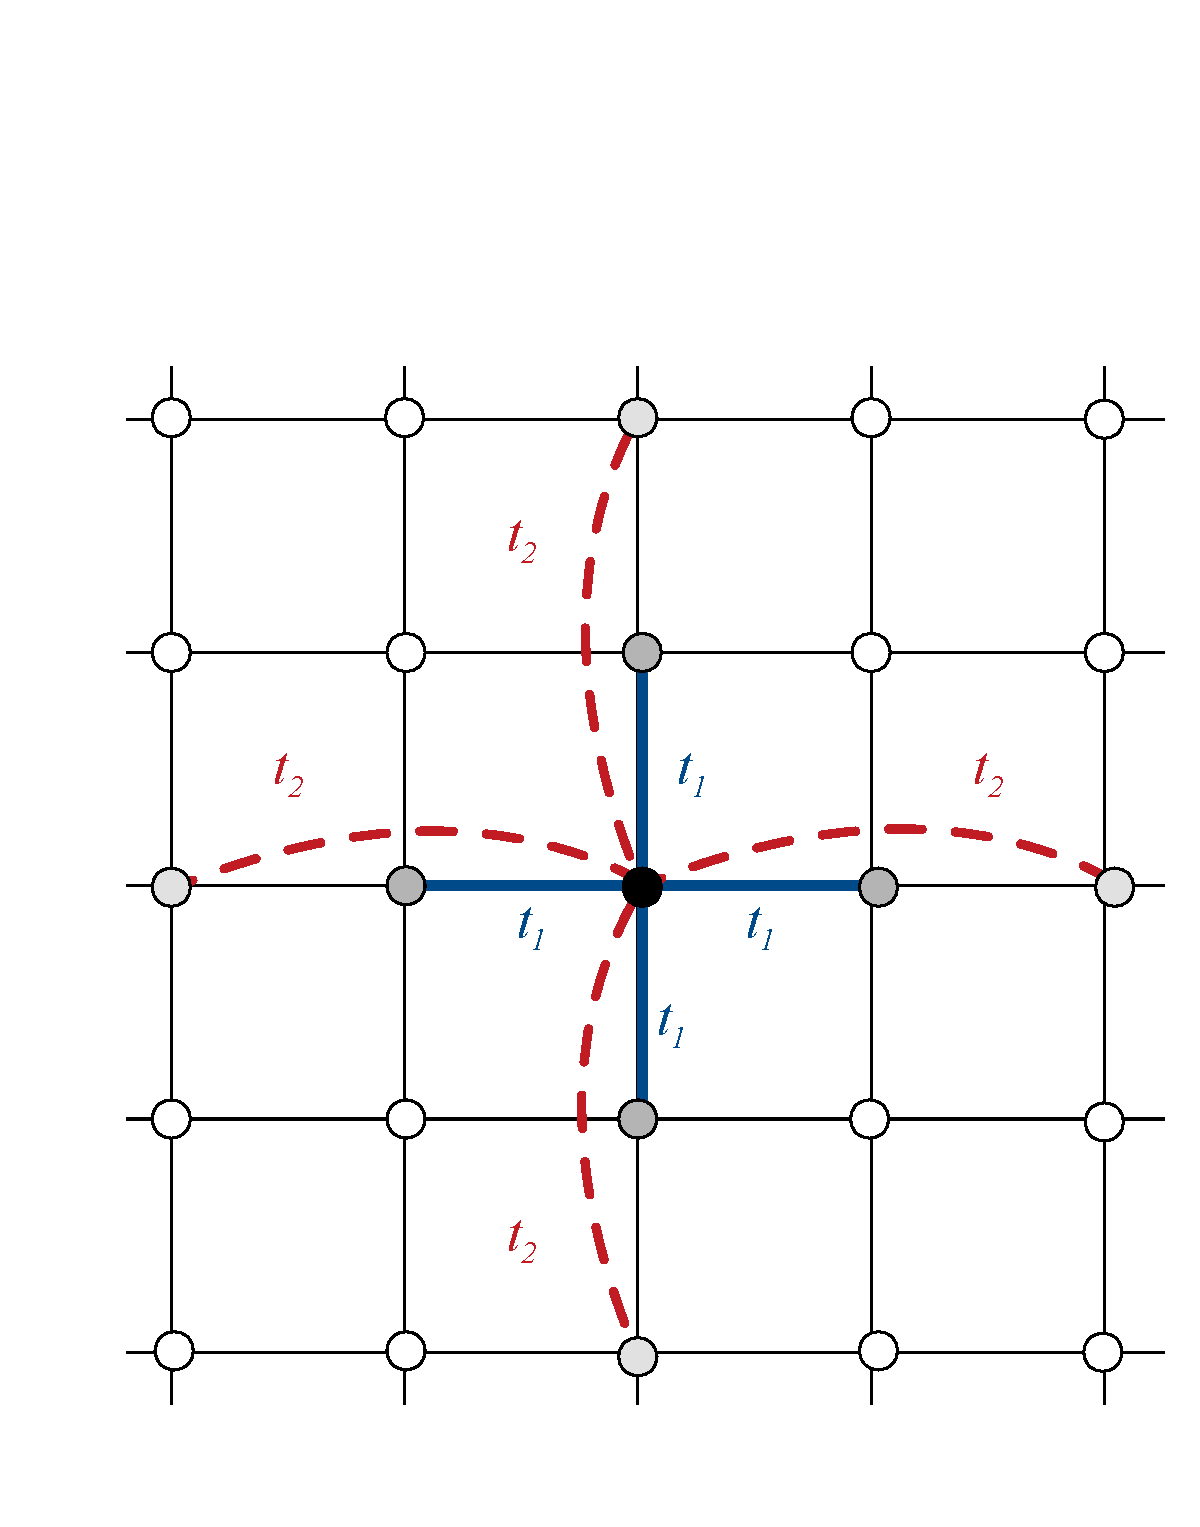
\includegraphics[width=3in]{quartic-hofstadter-hoppings-2.pdf}
\caption{\label{hoppings} Nearest-neighbor (NN) and next-nearest-neighbor hopping terms included in the hamiltonian (X). For the fine-tuned model, we set $t_2 = -t_1/4$.}
\end{figure}

\begin{figure}[thb]
\centering
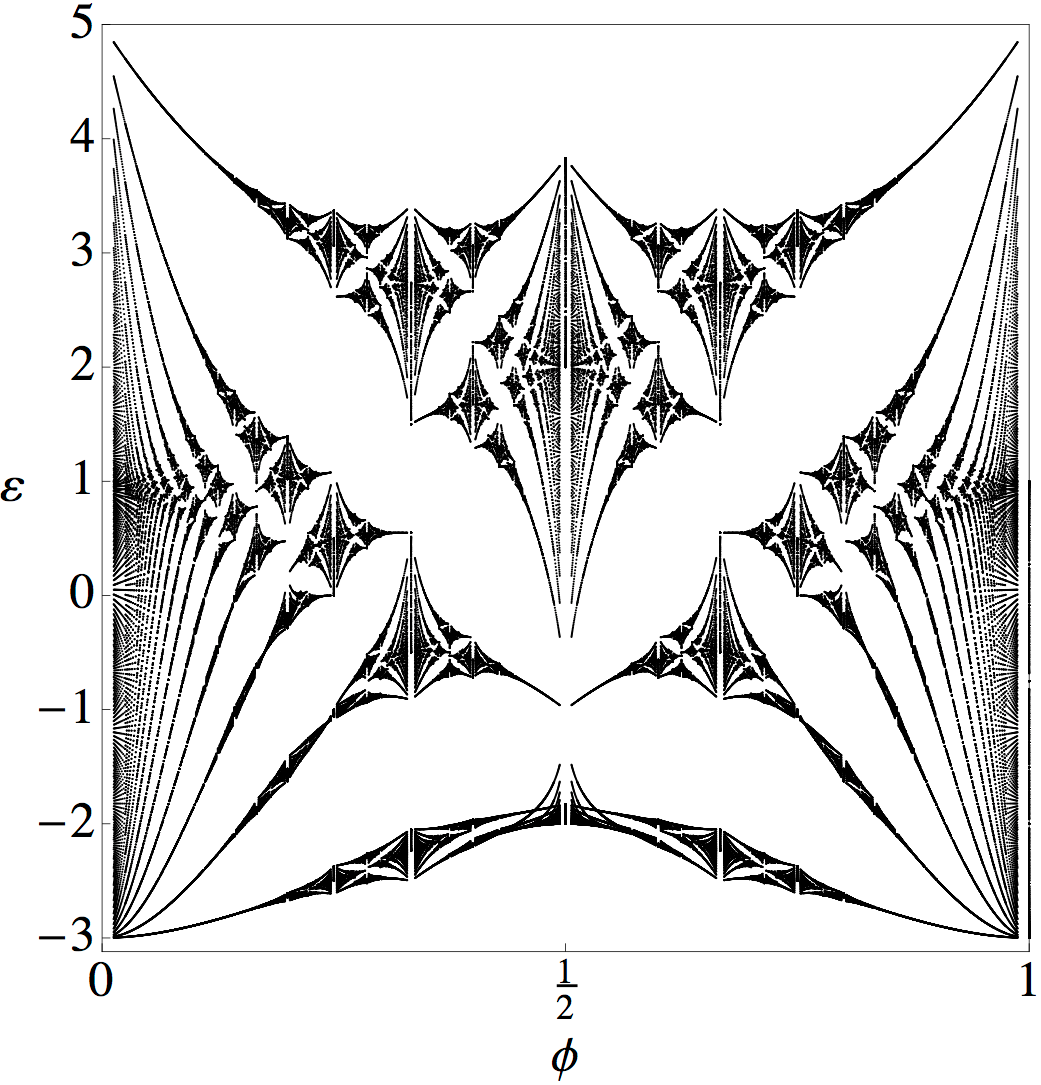
\includegraphics[width=3in]{quartic-butterfly-3.pdf}
\caption{\label{butterfly-plot} Energy eigenvalues of the hamiltonian (X) as a function of magnetic flux per elementary lattice plaquette $\phi = \hbar a^2/(e \ell^2) = P/Q \Phi_0$.}
\end{figure}

As in Section \ref{landau-levels} above, we can write this in terms of the hermitian generators of lattice translations,
\begin{align*}
H_0 = &-2t_1\left(\cos(\Pi_1) + \cos(\Pi_2)\right)\\ &- 2t_2\left(\cos(2\Pi_1) + \cos(2\Pi_2)\right)
\end{align*}
Replacing the cosine terms by their Taylor expansion, the terms lowest-order in the momenta are 
\begin{align*}
H_0 = &-4 t_1 - 4 t_2 + (t_1 + 4t_2) \left(\Pi_1^2 + \Pi_2^2\right) \\
&- \left(\frac{t_1}{12} + \frac{4}{3}t_2\right) \left(\Pi_1^4 + \Pi_2^4\right) + \ldots
\end{align*}
If we make the particular choice of hopping amplitudes $t_2 = -t_1/4$, then the quadratic terms vanish exactly, and we are left with an effective hamiltonian that is quartic in the momenta to lowest order (dropping additive constants):
\begin{align}
\label{hamiltonian-quartic-effective}
H_{\text{eff}} = \frac{t_1}{4} \left(\Pi_1^4 + \Pi_2^4\right).
\end{align}
The negative hopping amplitude could in principle be realized in optical lattice experiments by periodic ``shaking'' of the lattice. Unlike the Landau level hamiltonian, this hamiltonian does not have $SO(2)$ rotational symmetry, but it is symmetric under the square lattice isometry group $D_4$. 

As in the Landau level problem, we can choose a gauge and introduce Fock operators $a$, $a^{\dag}$ for the momentum/cyclotron degrees of freedom. For example, in the Landau gauge, the Fock operators are
\begin{align*}
a &= \frac{1}{\sqrt{2}\epsilon}\left(\Pi_1 - i\Pi_2\right)\\
a^{\dag} &= \frac{1}{\sqrt{2}\epsilon}\left(\Pi_1 + i\Pi_2\right).
\end{align*}
In terms of these operators,
\begin{align*}
H_{\text{eff}} = \frac{t_1\epsilon^4}{8}\left[a^4 + a^{\dag 4} + 6\left(a^{\dag}a + \frac{1}{2}\right)^2 + \frac{3}{2}\right].
\end{align*}

We numerically approximate this hamiltonian by working in a basis of LL eiegenstates ${\ket{n\text{-LL}}}$ staisfying $a^{\dag}a{\ket{n\text{-LL}}}=n{\ket{n\text{-LL}}}$ and truncating to a finite-dimensional subspace. This gives estimates for the cyclotron energies and overlaps with the Landau level states. We find good agreement between this truncated continuum approximation and exact numerical energy levels of lattice hamiltonian for small $\epsilon$.

We can study the spectrum of cyclotron orbits of this hamiltonian semiclassically by applying the Bohr-Sommerfeld quantization condition. In our notation this is
\begin{align*}
\oint\limits_{H=E_n} \Pi_1\, d\Pi_2 = 2\pi n,
\end{align*}
with the integral taken over a closed curve of constant energy in classical phase space. From this condition we find
\begin{align*}
E_n \sim n^2\phi^2, 
\end{align*}
in agreement both with the numerically-obtained, approximate spacing of the cyclotron levels, and with the quadratic dependence of $E$ on $\phi$ observed in the butterfly plot Fig \ref{butterfly-plot}.

\subsection{Effect of interactions}
[In progress]
The bands of our weak-field lattice hamiltonian correspond to cyclotron orbits that are distinct from Landau levels. However, we still expect that fractionally filling these bands with interacting particles will lead to FQH phases. To verify this, we numerically diagonalize the interaction hamiltonian projected to these bands

For both the Hofstadter model and our quartic model, the dispersion, Berry curvature, and Fubini-Study metric are all uniform over the MBZ up to exponentially small corrections\cite{Harper:2014vi,Bauer2016}. Geometric stability considerations\cite{Jackson2015} then suggest that the trace inequality $\expval{T}$ should provide information about the size of the many-body gap.

\subsection{Deviations from fine-tuning}
We now consider small perturbations away from the fine-tuned case $t_2 = -t_1/4$ by seting $t_2 = \left(-\frac{1}{4} + \delta\right)t_1$. In this case, instead of (\ref{hamiltonian-quartic-effective}) above, we have an effective hamiltonian with a quadratic term, ,
\begin{align*}
H_{\text{eff}} = t_1 \left[\left(\frac{1}{4}-\frac{4\delta}{3}\right)\left(\Pi_1^4 + \Pi_2^4\right) + 4\delta \left(\Pi_1^2 + \Pi_2^2\right)\right].
\end{align*}
If we make the $\epsilon$ dependence explicit by rescaling, we have
\begin{align*}
H_{\text{eff}} = \frac{t_1\epsilon^4}{4} \left[P_1^4 + P_2^4 + \frac{16\delta}{\epsilon^2} \left(P_1^2 + P_2^2\right)\right]
\end{align*}
to leading order. For a fixed $\delta$, we can always decrease the external magnetic flux density $B$, hence $\epsilon$, such that the quadratic term dominates, and our Chern bands are effectively Landau levels. However for a fixed $\epsilon$, $\delta$ may be small enough that the quadratic term can be treated as a perturbation to the quartic term, with perturbative parameter $16 \delta/\epsilon^2$ (with both $\epsilon,\,\delta$ small). A weak upper bound on the range of the small $\delta$ regime is given by enforcing $16 \delta/\epsilon^2 < 1$ or $\delta < $. Ref. \onlinecite{Aidelsburger:2014hm} observed the Hofstadter model in a system of ultracold atoms in an optical lattice, with effective values of $\phi = \hbar\epsilon^2/e = 2\pi/4$ and $J = t = (75\pm3s^{-1})h$. 

Numerical evidence suggests that the weak-field regime sets near $\phi/\Phi_0 \approx 1/15$, as measured by convergence of band-geometric quantities to their asymptotic values\cite{Bauer2016}.

We numerically calculate the value of the trace inequality of this model $\expval{T}$ for a few $\delta < 1/4$. Interestingly, the minimum of $\expval{T}$ occurs at finite $\delta$.

\section{Generalizations}
[In progress]
Although the previous section focused on a particular choice of hopping parameters, it is clear that in priciple one can engineer arbitrary inversion-symmetric band structures. The most general such model, following the discussion in Sec. \ref{landau-levels} is
\begin{align*}
H_{\text{eff}} = \sum_{j,k}t_{jk}\left(\Pi_1^{j}\Pi_2^{k} + \Pi_2^{k}\Pi_1^{j}\right)
\end{align*}

We of course may choose anisotropic hopping parameters $t_{jk}$ such that $C_4$ lattice symmetry that exchanges $x$ and $y$ directions is explicitly broken to $C_2$. For example, consider the hamiltonian
\begin{align*}
H_{\text{eff}} = h_{ab}\Pi_a \Pi_b + \lambda_{abcd} \Pi_a \Pi_b \Pi_c \Pi_d.
\end{align*}
In our order prescription, the coefficient tensors $h_{ab}$, $\lambda_{abcd}$ are chosen to be completely symmetric in their indicies.
By a $SL(2,\mathbf{R})$ transformation, we can diagonalize the effective mass tensor $h_{ab}$.


\section{Discussion}
[In progress]
We have show that one can construct models of Landau orbits in the continuum/weak-field regime that are distinct from Landau levels.

The models presented in this paper could provide a new regime in which to study the geometry of quantum Hall fluids 

\begin{acknowledgments}
The authors thank Tom Jackson for collaboration on related work and for his band geometry code. We also thank authors of the DiagHam package, which was used in this work.

\end{acknowledgments}
\bibliographystyle{apsrev4-1}
\bibliography{landau-orbits}


\end{document}


